\chapter{Framework implementation}
\label{chap:implementation}

The API, as described in chapter \ref{chapter:api}, and the decision making logic from chapter \ref{chap:deciding} was implemented into the ScalaAdaptive framework, a simple library that can be added to any Scala project and allows the programmer to utilize the adaptive decision making in his application.

In this chapter, we will go through the implementation of the framework, its basic architecture and the possibilities to extend it. We will also mention some decisions that had to be made during the implementation.

\section{Goals of implementation}

The main concerns upon implementing the framework were the following:

\begin{itemize}
	\item To separate the API from the selection logic
	\item To keep the framework strongly typed and use static type checking even in the internal parts of the code
	\item To make the framework as extensible as possible
	\item To keep the framework overhead as low as possible
	\item To keep the code well-organized, to minimize code duplication
\end{itemize}

\subsubsection{Development approach}

The main development approach was based on using the Scala language features to make the code simpler, easier to maintain and less error-prone. We tried to benefit from the functional approach whenever possible, while still keeping the high-level design object oriented. It leads to having the data and functionality separated in different classes. Inheritance is used only for implementing traits (except for some special cases, like the API function objects). All of the functionality-providing classes are used via corresponding traits, and thus communicating only through a simple and limited interface, which allows replacing them very easily. These trait-based building blocks are put together using composition and delegation patterns.

\subsubsection{Error handling}

The framework is designed so that the number of exceptions handled in the code was minimized. The ScalaAdaptive itself does not raise almost any exceptions in case of errors\footnote{The only exception being custom identifier validation in the function combination.}, and catches most of the exceptions from the libraries within to replace them with a None return value.

This approach is known from the functional programming and takes advantage of monadic operations over the \textit{Option monad}\footnote{In Haskell and other languages known as Maybe monad.}. The return values can be mapped over using the \textit{bind} operator, which allows smooth function chaining and the error propagation through the chain. More details can be found in the talk \cite{noauthor_railway_nodate}.

\section{Architecture overview}
\label{sec:architecture_overview}

This section will provide brief overview of the entire framework architecture and related decisions. More detailed description at the level of individual classes can be found in the documentation (see  \hyperref[attach:scaladoc]{attachments}).
%TODO: Documentation reference

\subsection{API architecture}
\label{subsec:api_architecture}

As briefly described in section \ref{subsec:api_implementation}, the public API of the framework is represented by a set of traits \inlinecode{AdaptiveFunction0}, ..., \inlinecode{AdaptiveFunction5}, which expose all the user accessible methods. Because only some of the methods depend on the number of input arguments, the part of the API that can be generalized was extracted into a common trait \inlinecode{AdaptiveFunctionCommon}, which is parametrized by the function type that extends it. 

\begin{figure}[h!]
	\captionsetup{justification=centering,margin=0.5cm}
	\centerline{\mbox{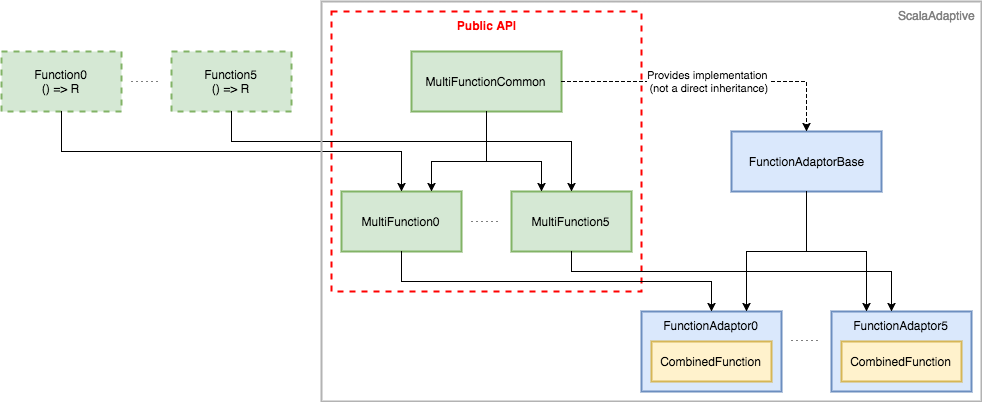
\includegraphics[width=140mm]{./img/inheritance_function_adaptors.png}}}
	\caption{Diagram showing the inheritance chain of AdaptiveFunctionN and related classes.}
	\label{fig:inheritance_function_adaptors}
\end{figure}

The \inlinecode{AdaptiveFunctionN} traits are implemented by \inlinecode{FunctionAdaptorN} classes that are directly inaccessible to the user, which allows us to modify or extend their internal API without changing the public API, thus maintaining backwards compatibility. The methods that can be implemented independently on the number of input arguments are extracted into an abstract class \inlinecode{FunctionAdaptorBase} that the other adaptors inherit from.

It would be quite impractical to manipulate with N different classes that represent the combined functions inside the internal parts of the framework. Therefore, the actual class holding the functions, \inlinecode{CombinedFunction}, is wrapped inside each one of the \inlinecode{FunctionAdaptorN} and is parametrized by the tuple type consisting of all the N arguments of the original function, and by the return type. All the functions are converted into functions of type \inlinecode{(TArgType) => TRetType} in the following way:

\lstset{style=Scala}
\begin{lstlisting}
val tupleFunction = (tupleArg) => function(tupleArg._1, ..., tupleArg._n)
\end{lstlisting}
	
The whole inner part of our framework works only with \inlinecode{CombinedFunction} types and therefore with functions of type \inlinecode{(TArgType) => TRetType}. Individual function adaptor classes perform the composition of the arguments into the tuple version before propagating the call further whenever a method depending on the argument number is invoked.

The figure \ref{fig:inheritance_function_adaptors} shows this inheritance and composition scheme.

The user of the framework will generate the instances using implicit conversion methods defined on an \inlinecode{Implicits} singleton, a part of the API that is described in \ref{subsec:api_implementation}. The actual conversions where the \inlinecode{FunctionAdaptorN} and the \inlinecode{CombinedFunction} instances get created will be wrapped inside another singleton object, \inlinecode{Conversions}, and the delegating calls will be done using a macro due to reasons explained later.

\subsection{Internal architecture}
\label{subsec:internal_architecture}

The simplified internal architecture can be seen in the figure \ref{fig:internal_architecture}. It shows the core chain that is executed when a combined function, represented as a \inlinecode{AdaptiveFunctionN} to the user, but internally stored as a \inlinecode{CombinedFunction} instance, is called.

\begin{figure}[h!]
	\captionsetup{justification=centering,margin=0.5cm}
	\centerline{\mbox{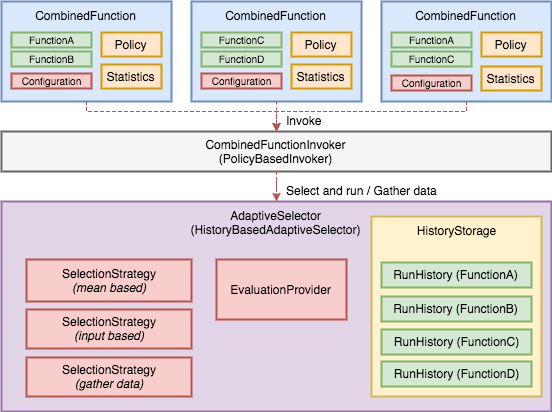
\includegraphics[width=140mm]{./img/internal_architecture.png}}}
	\caption{Diagram showing the internal architecture of the ScalaAdaptive framework.}
	\label{fig:internal_architecture}
\end{figure}


As we can see, there are two principal logic units participating in the process:

\begin{enumerate}
	\item \textbf{\inlinecode{CombinedFunctionInvoker}} \\
	Supposed to make a quick decision based on the policy of the combined function. It should either directly invoke one of the functions, or delegate the call to the \inlinecode{AdaptiveSelector}, and update the statistics of the combined function afterwards. It works only with the data directly stored in the \inlinecode{CombinedFunction} instance, it does not have any state or shared storage.
	\item \textbf{\inlinecode{AdaptiveSelector}} \\
	The key component of the framework, it receives a set of functions and an input, and it should decide which one of them to run and to execute it, evaluate the function run and return the result. The default implementation works with an abstract history storage (\inlinecode{HistoryStorage}), three selection strategies (\inlinecode{SelectionStrategy}) and an evaluation mechanism (\inlinecode{EvaluationProvider}).
\end{enumerate}

\section{Implementation options}

A few questions regarding the implementation arise from the basic architecture showed in section \ref{sec:architecture_overview}. We will provide a brief analysis before explaining the implementation details any further.

\subsection{History storage location}
\label{subsec:storing}

\inlinecode{HistoryStorage} is supposed to gather and store history data for all functions that are invoked using a combined function. The question is, where to save the data and how accessible to make it. We propose three variants.

\subsubsection{Local}

First option is to make the storage part of the \inlinecode{CombinedFunction} itself. In this case, the history data would, just like the statistics, be unique for every instance of the class, i.e. for every \inlinecode{AdaptiveFunctionN} created by the user. This has two consequences:

\begin{itemize}
	\item A function will have separate histories for every use in a combined function
	\item Every new instance of a combined function will have an entirely new history for all the functions
\end{itemize}

The second consequence might lead to some unexpected behavior - for example, if we create a combined function inside of a method call as described in section \ref{subsubsec:method_from_combined_func} and call it just once, it will have a clear history every time and will be useless:

\lstset{style=Scala}
\begin{lstlisting}
def processData(data: List[Int]): Int = 
  (impl1 _ or impl2 withStorage Storage.Local)(data)
\end{lstlisting}

Some use cases for this configuration exist, e.g. if we have a class that holds some immutable data and we keep executing some computations on the data, then a combined function defined as a field on this class with local storage will adapt specifically to the data of the class and does not need input based strategies.

\subsubsection{Global}

Another option is to store all the measured data globally, in a static area of the memory accessible from all contexts. This will allow to collect run data for functions faster and share them across all the combined functions, which usually leads to more informed and more precise decisions. This is usually the preferred approach for some business logic or utility methods in long-running services. A unique identifier has to be used to match the function history record with the actual function in the \inlinecode{CombinedFunction} class. The selection of the identifier will be discussed later.

\subsubsection{Persistent}

The biggest problem of the discussed storage locations is that the run history data are available only during a single run of the application. Whenever the application restarts, it will have to collect the data again. This might not be a problem for some long running services or daemons, but it is not very convenient for some tools or client applications with shorter lifecycle.

A solution to the problem is storing the data in a persistent storage, (e.g. HDD). We can do it in three different ways:

\begin{enumerate}
	\item Immediately persist each run history record
	\item Persist all of the records when the application terminates
	\item Buffer the history records and persist them in batches
\end{enumerate}

The first option seems like the best one, but it would lead to a series of I/O operations upon every invocation of a combined function. The added overhead of this solution could be dramatic. The second option, on the other hand, has no runtime overhead at all, but it requires a possibility to detect an application termination from our framework. JVM does not guarantee finalizers being called and relying on notifications from the user would complicate the API and be problematic in general. 

There is a mechanism in JVM called \textit{shutdown hooks} that allow the user to perform a custom action on shutdown (for more details see \cite{noauthor_jvmshuthooks_nodate}). It will, however, not be called when the application crashes. Additionally, it might be unexpected from a library to perform actions on shutdown and the delay that caused by persisting a lot of run data on a slow HDD (or even a network drive) could lead to the application being terminated immediately in some automatized environments.
Therefore, the third option was selected, as it leads to the runs being regularly saved and the I/O overhead is lower.

The persistence relies on the unique function identifier as well. There are additional problems connected to persisting the run history, namely:
\begin{itemize}
	\item Running multiple instances of the application at once (collisions on the persisted data file)
	\item Changes in the application code (outdated run data, changed identifiers, etc.)
	\item Having to deal with larger amounts of history data
\end{itemize}

\subsection{History storage function identifiers}
\label{subsec:function_identifiers}

As described in section \ref{subsec:storing}, we need some sort of identifier of the function to be able to store the run history data in a global or persistent storage. It does not make sense to use the references to the function objects, as new closure instances are created every time a lambda expression (or an eta-expanded method) is assigned, which would lead to having new history for each new instance, a behavior equivalent to local storage discussed in \ref{subsec:storing}.

%TODO: Reference an example?

This leaves us with three basic identifier options.

\subsubsection{Type name}

As explained in \ref{subsec:functiontypes}, functions in Scala are instances that extend the \inlinecode{FunctionN} trait. The default implementations are anonymous closure classes that are compiled from lambda expressions. Two different functions originate in two different lambda expressions and thus have two different type names, the ones that were generated and assigned by the compiler. The fully qualified type name can be used as the identifier of a function

Using the type names as unique identifiers is safe and straightforward. A small disadvantage is that they are not very readable, the compiler uses the name of the type that contained the lambda expression followed by sequential number. 

There is also a subtle danger connected - if we try to combine two different function that originated from the same lambda expression (the difference might be determined by the closure arguments), they will have the same identifier, thus sharing the same history, which is usually not desirable.

The next problem is that in case of persisting the run history, the closure classes might get renamed automatically upon recompiling. The compiler usually assigns the closure names sequentially, so this could happen by just inserting another lambda expression into the enclosing class code before the current one. Run history data might even get mixed up as the newly added lambda expression could have the former name of the original closure (by taking its position in the sequence).

Last but not least, If the \inlinecode{FunctionN} trait has a different than default implementation, the type name identification might fail - the trait can be implemented by a single class wrapping other values. In this case, all functions implemented by that class would share the run history.

\subsubsection{Method name}
\label{subsec:methodnameident}


The expected most common usage pattern of the framework is the one where the functions used with the \inlinecode{or} method are \textit{eta-expanded} methods (see \ref{subsubsec:apimethods}). There is a problem connected with methods when using the type name identifiers - every time a method gets eta-expanded, a new lambda expression with new type name is generated. In the following case, the \inlinecode{method1} would not have the same identifier in the two combined functions:

\lstset{style=Scala}
\begin{lstlisting}
val fun1 = method1 _ or method2
val fun2 = method1 _ or method3
\end{lstlisting}



It would be handy to use the method name as an identifier in such a case, which would lead to better readability and allow the same method used in different combined functions to have just one run history.

The problem is that at runtime, the implicit type conversion method or the \inlinecode{or} method will always get the already \textit{eta-expanded} function object with a compiled \inlinecode{apply} method holding the actual method call inside. The names have to be extracted at compile time, using the def macros (see \ref{sec:defmacros}). At the moment of the implicit conversion from \inlinecode{FunctionN} to \inlinecode{AdaptiveFunctionN} (as described in \ref{subsec:api_implementation}), the AST\footnote{Abstract syntax tree.} of the \inlinecode{FunctionN} expression can be examined - if it's a lambda expression containing one method call, the method name can be extracted. The exact process how to do so will be presented in a separate section.

\subsubsection{Custom identifier}
\label{subsubsec:custom_identifier}

In order to handle the specific cases where type name and method name identifiers do not distinguish correctly between different functions, there is also a possibility of choosing a custom, arbitrary identifier. This has to be triggered specifically by the user in the API and should be used in the cases where:

\begin{enumerate}
	\item User knows that the automatically assigned identifiers will not be sufficient
	\item User wants to replace default type identifier with custom identifier because of readability
\end{enumerate}

\section{Extracting method name from eta-expansion AST}
\label{sec:extracting_method_name}


In the description of the API in section \ref{subsec:api_implementation}, we introduced an implicit method that will perform the conversion from \inlinecode{FunctionN} to \inlinecode{AdaptiveFunctionN}. In order to extract the method name from potential uses of eta-expanded methods in this conversion, we will have to implement it in the following way:

\begin{enumerate}
	\item Replace the implicit conversion method by a def macro (see \ref{sec:defmacros}) and extract the conversion logic into a different, non-implicit method that allows explicitly setting the function identifier (in our case, the \inlinecode{Conversions} singleton object methods \inlinecode{toAdaptor()})
	\item Inside the implicit macro, analyze the AST and try to locate the eta-expansion method call
	\item If the method call is successfully found:
	\begin{enumerate}
		\item Generate the identifier expression as a \inlinecode{getTypeName} call on the target of the method call, concatenated with the method name
		\item Generate the conversion code with explicitly specified identifier expression
	\end{enumerate}
	\item Otherwise generate the conversion code with implicit identifier	
\end{enumerate}

The conversion is done using the \inlinecode{toAdaptor()} method with two overloads:
\begin{itemize}
	\item Accepting only the function - implicit identifier is used (type name of the closure)
	\item Accepting the function and a custom identifier - the identifier provided is used
\end{itemize}

\subsection{Eta-expansion AST format}

First step in the macro implementation has to be parsing the input AST and detecting patterns that are generated from eta-expansions by the compiler. Using the \inlinecode{printAst()} macro mentioned in \ref{subsec:buildingast}, the following facts were discovered:

\begin{itemize}
	\item The eta-expansion is already replaced by the equivalent code in AST, so it cannot be detected directly.
	\item The result of eta-expansion is a lambda expression (referred to as function literal in the AST).
\lstset{style=Dump}
\begin{lstlisting}
Function(...)
\end{lstlisting}
	\item The lambda expression is always wrapped in a block, being its return value.
	
\lstset{style=Dump}
\begin{lstlisting}
Block(
  List(...), 
  Function(...))
\end{lstlisting}	
	
	\item If the target of the invocation is either a constant or \textit{this}, it is captured in the lambda expression closure (i.e., the constant or \textit{this} is referenced directly from the function body).
	
	\item If the target of the invocation is a variable or a result of a more complicated expression, it is extracted to the enclosing block, its result is stored in a variable local to the block and then captured in the lambda expression closure. The following example shows how the target, originally an expression \inlinecode{this.getInstance()} on a \inlinecode{Class} class, was extracted into the block body.
	
\lstset{style=Dump}
\begin{lstlisting}
Block(
  List(
    ValDef(
      Modifiers(SYNTHETIC), 
      TermName("eta$0$1"), 
      TypeTree(), 
      Apply(
        Select(
          This(
            TypeName("Class")), 
          TermName("getInstance")), 
        List()))), 
  Function(...))
\end{lstlisting}

	\item The function node contains argument definition and the expression itself, which is a single application (method call).

\lstset{style=Dump}
\begin{lstlisting}
Function(
  List(
    ValDef(
      Modifiers(PARAM | SYNTHETIC), 
      TermName("arg"), 
      TypeTree(), 
      EmptyTree)), 
  Apply(...))
\end{lstlisting}
\end{itemize}

This has a few consequences for our case. First, we will look for functions with a body consisting from one method call. Secondly, we need to generate our conversion code (along with the method retrieval) into the block return value, because we need to be able to access the actual invocation targets that might exist only in the block (as the original expression was extracted and replaced by a local variable). The target and the method name will always be in the single Apply node representing the function body.

\subsection{Retrieving the target from the method call}

Now we need to go through the method call subtree and locate the invocation target. If the method does not accept any type arguments, the structure is quite simple:

\lstset{style=Dump}
\begin{lstlisting}
Apply(
  Select(
    ...invocation target expression..., 
    TermName("methodName")), 
  List(...function arguments...))
\end{lstlisting}

Where the \textit{invocation target expression} can have multiple forms based on the original expression, and can depend on the enclosing block variables. It is not, however, important for us, as we can work with the expression as whole. The function arguments are not needed either.

If the method is generic, the type arguments need to be applied in order to convert it to a function (which can't be generic). In this case, the tree gets a little more complicated:

\lstset{style=Dump}
\begin{lstlisting}
Apply(
  TypeApply(
    Select(
      ...invocation target expression..., 
      TermName("genericMethod")), 
    List(...type arguments...))), 
  List(...function arguments...))
\end{lstlisting}

The method call is wrapped in a TypeApply node before being invoked using the Apply node. The TypeApply node can be ignored in our case.

And the most complicated case we are going to analyze is when the method has some implicit arguments as well:

\lstset{style=Dump}
\begin{lstlisting}
Apply(
  Apply(
    TypeApply(
      Select(
        ...invocation target expression...,
        TermName("genericMethodImplicit")), 
      List(...type arguments...)), 
    List(...function arguments...)), 
  List(...implicit arguments...))
\end{lstlisting}

One more Apply node is added to the topmost level - the implicit arguments are applied after applying the actual function arguments. Their definition contains another nested block and lambda expression, but again, it is not important for our case. We just need to extract the invocation target and the method name, which can be both found in the Select node in one of the previous cases.

Note that there are situations where the eta-expansion might lead to more complicated trees, for example when used on methods with multiple argument lists. These are, however, cases which we are not going to support with the extraction.

\subsection{Generating the conversion}
\label{subsec:generate_conversion}

Supposing we have the invocation target expression and the method name, we need to create the identifier string expression that will be used in the manual \inlinecode{toAdaptor} invocation.

In order to extract the fully qualified name of the method call target, we need to generate the following expression:

\lstset{style=Scala}
\begin{lstlisting}
invocationTarget.getClass.getTypeName + ".methodName"
\end{lstlisting}

The AST representing this expression has to be wrapped in a construction application of \inlinecode{MethodNameIdentifier} class (it is a case class with automatically generated \inlinecode{apply()} method) to get the resulting identifier.

In all the cases, the \inlinecode{toAdaptor} method has to be generated to replace the macro function. The function literal from the original AST has to be passed in as the first argument, and optionally, the second argument containing the method name identifier can be provided if the extraction of the method name was successful.

The original tree in a simplified form can be seen in figure \ref{fig:original_eta_ast}.

\begin{figure}[h!]
	\captionsetup{justification=centering,margin=0.5cm}
	\centerline{
		\begin{forest}
			[Block
			[Statements
			[ValDef]
			]
			[Function]
			]
		\end{forest}
	}
	\caption{The original simplified eta-expansion AST.}
	\label{fig:original_eta_ast}
\end{figure}

We need to transform the block, keeping the definition in the statement part, but wrapping the \inlinecode{Function} into the \inlinecode{toAdapter} call, as shown in figure \ref{fig:transformed_eta_ast}.
	
\begin{figure}[h!]
	\captionsetup{justification=centering,margin=0.5cm}
	\centerline{
		\begin{forest}
			[Block
			[Statements
			[ValDef]
			]
			[Apply
			[toAdaptor]
			[ArgumentList
			[Function]
			[ExtractedIdentifierExpression]
			]
			]
			]
		\end{forest}
	}
	\caption{The simplfied eta-expansion AST after manually adding toAdaptor call.}
	\label{fig:transformed_eta_ast}
\end{figure}

\subsection{Extracting method overloads}

The approach that was described so far has one small issue - it does not recognize function overloads, so all the overloads share the same identifier.

 It would not be difficult to extract the actual number of arguments that the method is being invoked with and include it in the identifier. As for extracting their types, the situation gets a little complicated - the function literal is generated without argument type specification, the TypeTree is empty:

\lstset{style=Dump}
\begin{lstlisting}
ValDef(
  Modifiers(PARAM | SYNTHETIC), 
  TermName("i"), 
  TypeTree(), 
  EmptyTree)
\end{lstlisting}

This is a valid AST in Scala and can be generated in a lot of situations, for example:

\lstset{style=Scala}
\begin{lstlisting}
val function: (Int) => Int = { i => math.abs(i) + 1 }
\end{lstlisting}

In this case, the lambda expression does not have the type of its arguments specified either, because the compiler will infer it from the context in which the expression is used, in this case, from the type specifier of the variable it is being assigned to.

The compiler is able to infer the data type from the usage of the argument as well\footnote{The code snippet is correctly compiled by the Scala compiler, although some IDEs (namely IntelliJ IDEA 2016.3.4) are not able to infer the type and mark the code as incorrect.}:
\lstset{style=Scala}
\begin{lstlisting}
def method(i: Int): Int = ???
val function = { i => method(i) }
\end{lstlisting}

Note that the eta-expansion is guided by the same rules, so whenever expanding a method without overloads, the compiler infers the types by itself:
\lstset{style=Scala}
\begin{lstlisting}
def method(i: Int): Int = ???
val function = method
\end{lstlisting}

Upon expansion of a method with overloads, the resulting function type has to be provided either explicitly, or as an expected type in an expression (e.g. inside a method argument). The inference flow goes in the other direction in such a case:
\lstset{style=Scala}
\begin{lstlisting}
def method(i: Int): Int = ???
def method(s: String): Int = ???
val function: (String) => Int = method
def useFunction(fun: (Int) => Int): Unit = ???
useFunction(method)
\end{lstlisting}

As a consequence, at the time of syntax analysis, the types are not inferred yet and there is no way for us to find out which method overload is being called.

The method overloads therefore have to share the same identifier. If it leads to a problem, a type name or a custom identifier can be used in such a case.

\subsection{The conversion demonstration}

As a practical demonstration of the process described in this section, we are going to show the compile-time conversions that are done on a method identifier that is being \textit{eta-expanded} and converted into a \inlinecode{AdaptiveFunctionN}. Let's consider the following code:

\lstset{style=Scala}
\begin{lstlisting}
val combined = target.method _ or function
\end{lstlisting}

We will follow the conversions that the compiler and our macro perform on the \inlinecode{target.method \_} expression\footnote{The actual changes are performed on the AST level, we will show them in corresponding Scala code for simplicity.}:

\begin{enumerate}
	\item The explicit \textit{eta-expansion} is performed:
	\lstset{style=Scala}
	\begin{lstlisting}
{ () => target.method() }
	\end{lstlisting}
	\item The implicit conversion is applied:
		\lstset{style=Scala}
	\begin{lstlisting}
Implicits.toAdaptiveFunction0({ () => target.method() })
		\end{lstlisting}
		\item The macro \inlinecode{toAdaptiveFunction0} is executed and expanded:
		\lstset{style=Scala}
		\begin{lstlisting}
Conversions.toAdaptor({ () => target.method() }, MethodNameIdentifier(this.getClass.getName + ".method"))
		\end{lstlisting}
\end{enumerate}

The final state shows the code that will be present in our compiled program and will be executed.

\subsection{Macros in the combining method}

In the section \ref{subsubsec:apimethods}, we explained why the \inlinecode{or} method has to accept an argument of \inlinecode{FunctionN} type instead of \inlinecode{AdaptiveFunctionN}. This does not seem to cause any trouble as we can manually convert \inlinecode{FunctionN} into the \inlinecode{FunctionAdaptorN} inside the method body. With the macro expansion, however, we run into problems. Image we do it the following way:
\lstset{style=Scala}
\begin{lstlisting}
def or(fun: (T1) => R) = orAdaptiveFunction(Implicits.toAdaptiveFunction1(fun))
\end{lstlisting}

The  \inlinecode{toAdaptiveFunction1} method is a macro - it gets executed at compile time, and it receives the argument AST as its input. In this case, an AST that consists of the \inlinecode{fun} identifier. We have no way to find out, where this function will be called from and with which arguments, so in order to extract the method name, we need to convert the entire \inlinecode{or} function to a macro which will generate the conversion code in the same manner as described in section \ref{subsec:generate_conversion}, and then wrap it in the internal \inlinecode{orAdaptiveFunction} code.

This does not require any extra AST manipulations, only one method call generation. It does, however, mean a complication for us, as the macros cannot be called virtually. The macro definition therefore has to be a part of the \inlinecode{AdaptiveFunctionN} API trait, breaking somehow the encapsulation of the implementation. Fortunately, it does not perform any actions by itself, only replaces the \inlinecode{or} call with a conversion and an \inlinecode{orAdaptiveFunction} call, which is, again, a virtual method defined on the trait without implementation and therefore encapsulated.

\subsection{Extraction evaluation}

In order to evaluate the method name extracting solution presented throughout this section, we converted some expressions with function values to corresponding \inlinecode{AdaptiveFunctionN} types using the macro approach. Table \ref{tab:method_extraction_results} shows the results. Note that the package prefixes were omitted from the method names for simplicity, the actual identifiers contain fully qualified names. The conversion was performed in the scope of a \inlinecode{NameTest} singleton object.

% Please add the following required packages to your document preamble:
% \usepackage{booktabs}
\begin{table}[h!]
	\captionsetup{justification=centering,margin=0.5cm}
	\bgroup
		\begin{center}
	\begin{tabular}{ll}
		\toprule
		\textbf{Expression}             & \textbf{Assigned method name}              \\ \midrule
		\inlinecode{method \_}                                             & NameTest\$.method                   \\
		\inlinecode{genericMethod{[}Int{]} \_}                             & NameTest\$.genericMethod            \\
		\inlinecode{Singleton.quickSort \_}                         & NameTest\$Singleton\$.quickSort \\
		\inlinecode{variableSorter.quickSort \_}                           & Sorter.quickSort                            \\
		\inlinecode{getSorter.quickSort \_}                                & Sorter.quickSort                            \\
		\inlinecode{new Sorter().quickSort \_}                            & Sorter.quickSort                            \\
		\inlinecode{new GenericClass{[}Int{]}().foo \_}              &   GenericClass.foo                         \\
		\inlinecode{(i: Int) =\textgreater{} method(i)}                  &   N/A (Closure name used)                                        \\
		\inlinecode{(i: Int) =\textgreater{} method(i + 1)}                & N/A (Closure name used)                                        \\
		\inlinecode{function}                                                 &   N/A (Closure name used)                                        \\ \bottomrule
	\end{tabular}
\end{center}
\egroup
\caption{The method names extracted from expressions during their conversion to combined functions.}
\label{tab:method_extraction_results}
\end{table}

As we can see, the method name extraction succeeded in all the \textit{eta-expansion} cases and did not get confused even by a direct method call within a lambda expression.

\section{Module implementation}
\label{sec:module_impl}

All the modules mentioned in \ref{subsec:internal_architecture} are abstract traits with replaceable implementations, that are put together using composition. The API classes have to be able to access the composed and active implementations at the moment of invocation. For this reason, a singleton Scala object \inlinecode{AdaptiveInternal} was introduced and holds the following composed modules:

\begin{itemize}
	\item \inlinecode{AdaptiveSelector} with global storage
	\item \inlinecode{AdaptiveSelector} with persistent storage
	\item \inlinecode{CombinedFunctionInvoker}
\end{itemize}

We will briefly introduce the implementations of these modules and the parts that they are composed from.

\subsubsection{CombinedFunction}

The \inlinecode{CombinedFunction} is the main data class representing a function with multiple implementations in ScalaAdaptive. It is basically a data holder class, the important functionality was separated to be easily replaceable. It gets created and modified when a user of the framework manipulates with the \inlinecode{AdaptiveFunctionN} API type. Part of its attributes are immutable, representing the configuration and default setup of the function, and part of its attributes are mutable, holding its state in the invocation process.

It contains the following immutable data:

\begin{itemize}
	\item Set of functions that it is combined from (wrapped into the tuple form, see \ref{subsec:api_architecture})
	\begin{itemize}
		\item	Each function holds up to two identifiers - one based on the closure type name, the other being either a method name or a custom name, depending on the creation process (see \ref{subsec:function_identifiers})
	\end{itemize}
	\item \textit{Descriptor function} (wrapped into the tuple form), see \ref{sec:input_based_strategies}
	\item \textit{Group selector} function (wrapped into the tuple form), see \ref{subsubsec:group_selection}
	\item Function configuration defined by the user, will be described later in more detail
\end{itemize}

And the following state representing data:

\begin{itemize}
	\item Function statistics (separately for each group, see \ref{subsec:statistical_data})
	\item Current policy (separately for each group, see \ref{sec:policies})
	\item Analytics data - full list of all the selections and their results
\end{itemize}

In case of the local storage setup, the instance also has to contain its own \inlinecode{AdaptiveSelector} that holds the local \inlinecode{HistoryStorage}.

\subsubsection{CombinedFunctionInvoker}

It has access to the state of the \inlinecode{CombinedFunction} and its basic implementation does the following:

\begin{itemize}
	\item Evaluate current policy using the statistics of the combined function
	\item According to the result either invoke directly the function which is accessible through the statistics (the last one and the most selected one) in case of \inlinecode{UseLast} or \inlinecode{UseMost} results , or pass the decision onto the \inlinecode{AdaptiveSelector} in case of \inlinecode{SelectNew} or \inlinecode{GatherData} results
	\item Update the function statistics
\end{itemize}

The \inlinecode{AdaptiveSelector} is accessed either through the \inlinecode{CombinedFunction} itself for the local storage setup, or using the singleton object \inlinecode{AdaptiveInternal} in case of global or persistent setup.

\subsubsection{AdaptiveSelector}

A module which is supposed to select one of given options to run, and to evaluate the run. It is parametrized with \inlinecode{TMeasurement} type, which represents the data measured from the function run. By default, a \inlinecode{Long} type for run time measured is used. It supports two basic operations - \textit{selectAndRun} and \textit{gatherData}, which correspond to the policy results. Both of these operations have also an option with delayed measurement (see \ref{subsec:delayed_measuring}).

The implementation \inlinecode{HistoryBasedAdaptiveSelector} contains the general chain described in \ref{sec:selection_and_invocation_process}. It uses a \inlinecode{HistoryStorage} to store and retrieve the run data of individual functions. In addition, it holds three \inlinecode{SelectionStrategy} instances, one for gathering new data, one for the input based selection, and one for the mean based selection. One of these three instances is used to select the function to run, which is then executed using an \inlinecode{EvaluationProvider}. The measurement retrieved is added to the history and the result is returned, along with a performance benchmark including execution and overhead times (independent on the actual measurement, always based on wall-clock times) for the function statistics update. Figure \ref{fig:history_based_selector} shows the entire process.

In case of the operations with delayed measurement, the function run is not evaluated, an \inlinecode{InvocationToken} is generated instead. The token holds a callback to the \inlinecode{AdaptiveSelector} and whenever used to invoke some function, it will use the \inlinecode{EvaluationProvider} to evaluate the run and store the data to the corresponding history record.

Note that the \inlinecode{SelectionStrategy} for gathering new data should select a function for which data are needed the most at the moment instead of optimizing the performance.

\begin{figure}[h!]
	\captionsetup{justification=centering,margin=0.5cm}
	\centerline{\mbox{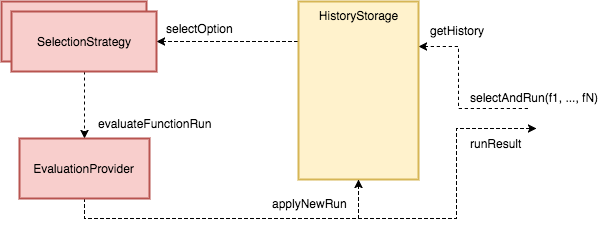
\includegraphics[width=100mm]{./img/history_based_selector.png}}}
	\caption{Diagram showing the HistoryBasedAdaptiveSelector execution path.}
	\label{fig:history_based_selector}
\end{figure}

\subsubsection{HistoryStorage}

A type with a map-like interface based on the concepts from section \ref{subsec:storing_evaluation_data} - it is supposed to hold the historical measurement vectors represented by \inlinecode{RunHistory} instances for each combination of function and input group. A key composed of a function identifier and a group identifier is used to access the histories.

There are two implementations in the framework:

\begin{itemize}
	\item\inlinecode{MapHistoryStorage} - stores the histories in memory
	\item\inlinecode{PersistentHistoryStorage} - a wrapping storage that delegates the calls to an internal \inlinecode{HistoryStorage}, and, in addition, it serializes every new run using a \inlinecode{HistorySerializer} and if asked for a history that is not present in the underlying storage, it tries to deserialize it using the same class
\end{itemize}

The \inlinecode{HistorySerializer} has two basic implementations, one for direct serialization, and one for buffered serialization. The data are stored into a file, one per function, and the format, root directory and file name pattern are fully customizable. There is no list of these history containing files anywhere - when trying to deserialize a function, a file with corresponding name is checked for existence. This means that the individual function histories are deserialized one by one, at the moment of the first invocation of a combined function that contains them, which might cause a delay in the first execution.

\subsubsection{RunHistory}
\label{subsubsec:run_history}

\inlinecode{RunHistory} represents the vector of historical measurement results and other details about a function run. The interface is designed to support immutable solution - the appending methods always return an instance of the same type, which might or might not be the same object depending on the implementation. The interface provides some basic operations on the history, allows iteration over the data and appending new data (always at the end). 

Apart from that, it also has some methods to directly provide precomputed data for some of the selection strategies in order to support caching. These supporting methods can always be computed using the data available, and if the implementation of \inlinecode{RunHistory} does not support the caching or precomputation, there are \textit{mixin} traits (see section \ref{sec:linearization_mixins}) with default implementations available.

The provided implementations of \inlinecode{RunHistory} can be chained using the \textit{Decorator} pattern to modify the behavior. The basic implementations are the following:
\begin{itemize}
	\item \inlinecode{FullRunHistory} - stores all runs in an \inlinecode{ArrayBuffer}, is mutable
	\item \inlinecode{ImmutableFullRunHistory} - stores all runs in an immutable \inlinecode{List}, is a little slower in general
\end{itemize}

These instances can be wrapped in the following decorator classes:
\begin{itemize}
	\item \inlinecode{LimitedRunHistory} - limits the maximum number of stored items, whenever it reaches maximum, it throws the older half of all the records away
	\item \inlinecode{CachedStatisticsRunHistory} - stores the statistical data about the run items, speeds up the t-test strategy (see \ref{subsec:t_test_multiple})
	\item \inlinecode{CachedGroupedRunHistory} - stores average evaluation data for each \textit{run selector}, speeds up the local regression strategy (see \ref{subsec:local_regression})
	\item \inlinecode{CachedRegressionRunHistory} - stores the linear regression model built upon all the run items, speeds up the linear regression strategy (see \ref{subsec:simple_linear_regression})
\end{itemize}

The \inlinecode{LimitedRunHistory} wrapper should always be used, as it can prevent unexpected out-of-memory exceptions in the program run, as the base run history implementations have no size limits.

\subsubsection{SelectionStrategy}
\label{subsubsec:selection_strategy_impl}

Very simple trait that represents the selection strategies described in detail in sections \ref{sec:input_based_strategies} and \ref{sec:mean_based_strategies}. The implementations should be stateless and should work only with the \inlinecode{RunHistory} records that it receives (in order not to mix together decisions about two separate history storage locations). The strategy implementations often have a customizable fallback strategy that is used in cases where the current strategy is not able to make a decision, as described in section \ref{subsec:solving_decision_failures}.

The strategies are parametrized by the \inlinecode{TMeasurement} type of the function run evaluation. All of the implemented strategies work with function run time represented either directly by \inlinecode{Long} or by a type viewable as \inlinecode{Numeric}.

The mean based strategies consist of the following classes:
\begin{itemize}
	\item \inlinecode{TTestSelectionStrategy} - implements the t-test strategy described in section \ref{subsec:t_test_multiple}, uses \cite{noauthor_apachemath_nodate} to compute the p-value.
	\item \inlinecode{UTestSelectionStrategy} - implements the u-test strategy described in section \ref{subsec:u_test}, uses \cite{noauthor_apachemath_nodate} to compute the test statistics.
\end{itemize}

The implemented input based strategies are:
\begin{itemize}
	\item \inlinecode{RegressionSelectionStrategy} - implements the linear regression strategy as described in section \ref{subsec:simple_linear_regression}, uses the \cite{noauthor_apachemath_nodate} to compute the regression

	\item \inlinecode{LoessInterpolationSelectionStrategy} - implements the local regression strategy from section \ref{subsec:local_regression}, uses the \cite{noauthor_apachemath_nodate} for the interpolation
\end{itemize}

In addition, some complementary supporting were added:
\begin{itemize}
	\item \inlinecode{WindowBoundSelectionStrategy} - a wrapper strategy that limits the history records to a flexible window as described in sections \ref{subsec:window_bound_regression} and \ref{subsec:window_bound_t_test}
\item \inlinecode{LowRunAwareSelectionStrategy} - if any of the functions has less than a specified number of history records, uses one strategy, otherwise, uses a different strategy
\item \inlinecode{LeastDataSelectionStrategy} - uses the function with least historical runs
\end{itemize}

The common pattern is to use the \inlinecode{LowRunAwareSelectionStrategy} as the topmost strategy in the composition to postpone the decision process until some data are ed, the \inlinecode{LeastDataSelectionStrategy} as the fallback strategy, and to have one of the actual input based or mean based strategies in the middle, optionally wrapped in the window-bound class. The \inlinecode{LeastDataSelectionStrategy} is also recommended to be used as the strategy for the \textit{gather data} operation of \inlinecode{AdaptiveSelector}.

\subsubsection{EvaluationProvider}

With a goal of potentially supporting larger variety of possible function evaluation data, the selected function is always executed using an implementation of \inlinecode{EvaluationProvider}, which is supposed to run the function and to evaluate it, and return both the result of the function and the evaluation data in the form of \inlinecode{TMeasurement}. The default implementation simply measures the wall-clock time of the function run.

\section{User interaction and customization}

The basic behavior of the combined functions can be changed in two ways:
\begin{itemize}
	\item Each combined function can have the most basic features configured individually
	\item The whole framework can be re-configured and customized
\end{itemize}

\subsection{Combined function setup}
\label{subsec:function_setup}

As the basic API designed in chapter \ref{chapter:api}, i.e. the \inlinecode{or} method used to create new combined functions, does not allow directly setting the function behavior, a simple configuration API has to be added. In compliance with the DSL-like \inlinecode{or} chaining, the configuration was made possible via special methods on the \inlinecode{AdaptiveFunctionN} type that allow chaining as well\footnote{In the \textit{builder}-style pattern, by returning the same type.} and are also meant to be used like operators. The combined function definition including the configuration can be very fluent and natural:

\lstset{style=Scala}
\begin{lstlisting}
val sort = standardSort _ or selectionSort by (_.size) selectUsing Selection.InputBased storeUsing Storage.Global
\end{lstlisting}

\subsubsection{Input descriptor and group selector}

The most important part of the configuration API are the \inlinecode{by} and \inlinecode{groupBy} methods. The first allow the user to specify the \textit{descriptor function}, i.e., function describing how to extract an \textit{input descriptor} from the input (see \ref{subsec:input_in_selection}). A function of type \inlinecode{(T1, ..., TN) => Long} is used for that, where \inlinecode{T1, ..., TN} are the arguments of the \inlinecode{AdaptiveFunctionN}. 

The second method expects a \textit{group selector}, which assigns the input to a certain group (see \ref{subsubsec:group_selection}). It should receive a function of type \inlinecode{(T1, ..., TN) => Group}.

\subsubsection{Function configuration}

Additional behavior can be modified for the combined function. The choice is based mostly on selecting which one of multiple implementation options should be used with given function. In the \inlinecode{AdaptiveInternal} singleton, we hold two implementations of \inlinecode{AdaptiveSelector}, one with persistent history storage, the other without. Each of these two implementations then includes two instances of  \inlinecode{SelectionStrategy}, one for input based and one for mean based selection.

The function configuration methods and possible values are the following:

\begin{itemize}
	\item \inlinecode{storeUsing} - represents the history storage options as described in section \ref{subsec:storing}
	\begin{itemize}
		\item \inlinecode{Global} - uses the shared \inlinecode{AdaptiveSelector} without persistent storage
		\item \inlinecode{Persistent} - uses the shared \inlinecode{AdaptiveSelector} with persistent storage
		\item \inlinecode{Local} - creates a new instance of \inlinecode{AdaptiveSelector} locally in the function object
	\end{itemize}
\item \inlinecode{selectUsing}
\begin{itemize}
	\item \inlinecode{InputBased} - uses the input based strategy in \inlinecode{AdaptiveSelector}
	\item \inlinecode{MeanBased} - uses the mean based strategy in \inlinecode{AdaptiveSelector}
	\item If none is specified, uses the input based strategy if the \textit{descriptor function} is set and the mean based strategy otherwise
\end{itemize}
\item \inlinecode{limitedTo} - allows to specify the maximum age of the history records to be used in the selection process, as described in \ref{subsec:limiting_record_age}
\item \inlinecode{asClosures} - represents the history storage identifier choice as described in section \ref{subsec:function_identifiers}
\begin{itemize}
	\item \textit{true} - always uses closure type names as the function identifiers
	\item \textit{false} - uses either method names or custom names as the function identifiers if available
\end{itemize}
\item \inlinecode{withPolicy} - allows to specify the starting policy for the function, as described in \ref{sec:policies}
\end{itemize}

The user is expected to specify this configuration with most of the combined functions. The default values are determined by the framework configuration, except for the selection strategy choice, which is defaulted to input based if the \textit{descriptor function} is provided for the combined function and to mean based otherwise.

\subsection{Logging, analytics and control access}

There are two basic mechanisms for the user of the framework to observe its functionality - logging and analytics.

\subsubsection{Logging}

Logging is performed by multiple parts that are involved in the selection process. An instance of the simple \inlinecode{Logger} trait held in the \inlinecode{AdaptiveInternals} and passed around to other modules is used for that purpose. The provided implementation of loggers are \inlinecode{ConsoleLogger}, \inlinecode{FileLogger} and \inlinecode{EmptyLogger}, where the last one does not actually save the logs anywhere, and is used by default to limit the overhead.

Replacing \inlinecode{EmptyLogger} with one of the other types will lead to detailed output describing each invocation of every combined function, which can be used to trace eventual problems with the framework behavior.

\subsubsection{Analytics and control access}
\label{subsubsec:analytics}

To provide a more systematic and technical access of the framework behavior, a simple set of methods was made accessible on the \inlinecode{AdaptiveFunctionN} type by extending the \inlinecode{AdaptiveFunctionControl} and \inlinecode{AdaptiveFunctionAnalytics} traits:

\begin{itemize}
	\item \inlinecode{train} - trains the combined function on a given set of inputs (by executing all of the functions on each of the inputs and storing the results)
	\item \inlinecode{flushHistory} - flushes the entire run history of given function (in the corresponding history storage)
	\item \inlinecode{setPolicy} - sets the current policy of the function to a custom one
	\item \inlinecode{resetPolicy} - sets the current policy of the function to the starting one
	\item \inlinecode{getAnalyticsData} - retrieves analytics data regarding the function history
\end{itemize}

The analytics data represent a way of monitoring the decisions of the selection process for each combined function. It contains a complete set of records of previous runs, each one holding the identifier of the selected function, the \textit{input descriptor}, run time and the overhead time spent on the selection. The data can either be analyzed directly in the application by processing these records, or can be easily serialized into a CSV file.

Note that the analytics data collection is relies on the \inlinecode{AnalyticsCollector} trait. Again, we provide two implementations, \inlinecode{BasicAnalyticsCollector} that collects all the data mentioned, and \inlinecode{EmptyAnalyticsCollector}, that does not collect anything. The empty variant is default in order to minimize the overhead of the framework. In case the user has a need of the analytics data from his application, he can enable the collection by replacing the collector.

\subsection{Framework configuration}
\label{subsec:framework_config}

In section \ref{sec:module_impl}, we mentioned a variety of building blocks that the main parts of the framework are composed of, and the possibility to use multiple implementation to change the behavior of the entire system. This is the more advanced part of the configuration and it requires manipulation with the actual implementations.

As explained earlier, all the shared and commonly accessible functionality is held inside the singleton object \inlinecode{AdaptiveInternal}. This object can be initialized using an \inlinecode{initialize()} method on a publicly accessible singleton \inlinecode{Adaptive}. The static description of the composition of the implementations that is followed in this process is provided by the \inlinecode{Configuration} trait. This can be thought of as a composition root of the whole system - it has to provide factory methods for all the building blocks used. In addition, it has an abstract type member \inlinecode{TMeasurement} that determines the type of the evaluation data used throughout the whole framework.

%TODO: Add ref to http://docs.scala-lang.org/tutorials/tour/abstract-types.html

The implementation of the \inlinecode{Configuration} trait has to provide a specific \inlinecode{TMeasurement} type and the factory methods that rely on the type. Note that the \inlinecode{AdaptiveSelector} trait and its methods do not depend on the \inlinecode{TMeasurement}, only its implementation does, so the type of the evaluation data does not leak outside of the composition root. As a result, the actual type can be changed at runtime by simply replacing the \inlinecode{AdaptiveSelector} instance.

The \inlinecode{Configuration} can be created by the user himself, using either a combination of provided implementation or his custom implementations. Alternatively, one of the predefined \inlinecode{Configuration} traits with some basic settings already implemented can be utilized:

\begin{itemize}
	\item \inlinecode{BaseConfiguration} - provides basic configuration of some of the types that do not depend on the \inlinecode{TMeasurement}
	\item \inlinecode{BaseLongConfiguration} - sets the \inlinecode{TMeasurement} type to \inlinecode{Long} and adds basic configuration of some of the types that depend on it
\end{itemize}

These traits have to be extended to define the unimplemented values.

\subsubsection{Configuration blocks}
 To simplify the configuration process when working with existing implementations and to hide the initialization details from the user, a concept called \textit{configuration blocks} was introduced. 
 
 \textit{Configuration blocks} are \textit{mixin} traits (see section \ref{sec:linearization_mixins}) that provide implementation for just one (or a few) functions from the \inlinecode{Configuration} trait, setting up part of the framework in given way. The user of the framework can then define the configuration by creating an anonymous class extending the base configuration along with desired \textit{configuration blocks}. Thanks to the fluent and simple syntax of Scala, this concept is very expressive and easy to use. The compile-time check will automatically alert the user if the combination of block does not cover some required method.
 
 In addition, some blocks can be parametrized. The parameters are always protected read-only attributes of the block trait that usually have default implementation (i.e. value), but can be overridden. It fits easily into the anonymous class usage pattern, as the new parameter values for all the blocks can simply be stated in the body of the class. Blocks can share a parameter by inheriting it from the same base trait - in such a case, it is impossible to set different values for different blocks.
 
 Some blocks call the parent implementation of the factory method to wrap its result into a different type. An example is the \inlinecode{CachedRegressionStorage}, which creates a wrapper for caching the linear regression model atop of the \inlinecode{RunHistory} provided by its parent (for information about the wrappers see \ref{subsubsec:run_history}). The parents in the configuration inheritance chain are determined using \textit{linearization} (see section \ref{sec:linearization_mixins}). According to the rules, we have to be careful when mixing in a block with implementations and a wrapping block at the same time - the block with implementation have to be listed before the wrapping block in the extensions list.
 
 The whole configuration can look the following way:

\lstset{style=Scala}
\begin{lstlisting}
val config = new BaseLongConfiguration
  with DefaultHistoryPath
  with RunTimeMeasurement
  with WindowBoundRegressionInputBasedStrategy
  with UTestMeanBasedStrategy
  with CachedRegressionStorage
  with CachedStatisticsStorage
  with FileLogging {
  override val maximumNumberOfRecords = 20000
  override val alpha = 0.25
  override val logFilePath = "./adaptive/log.txt"
}

Adaptive.initialize(config)
\end{lstlisting}

List of all the configuration blocks available along with their parameters can be found in appendix REF.

%TODO: ADD THE APPENDIX / ATTACHMENT REFERENCE!

\subsubsection{Default configuration}

A special class for the default configuration was created, which is used to initialize the ScalaAdaptive framework at the beginning of the application run and which specifies the implementations that are used if the user does not provide his configuration.

Based on the results observer in section \ref{sec:strategy_comparison}, we decided to include the t-test selection strategy with cached statistics as the mean based strategy, and the window-bound linear regression as the input based strategy.

The default configuration can be extended with any of the configuration blocks as well:

\lstset{style=Scala}
\begin{lstlisting}
val config = new DefaultConfiguration with ConsoleLogging
\end{lstlisting}

\subsection{Extending the framework}

The framework can be simply extended without actually modifying it by creating custom implementations of some of the traits that are used by the invocation and selection process, and by supplying it to the \inlinecode{Adaptive} initialization using a custom configuration, as described in \ref{subsec:framework_config}.

An overview of the areas that are the simplest and most useful to extend will follow.

\subsubsection{Selection strategies}

A new selection strategy can be created by extending the \inlinecode{SelectionStrategy} trait and by providing the implementation as either input based or mean based selection strategy. The trait itself is technically a single function corresponding to the algorithm mentioned in \ref{subsec:selecting_function}, which is given a sequence of function run histories and an input descriptor and is supposed to return the key (function identifier and group identifier) of the function with best expected performance:

\lstset{style=Scala}
\begin{lstlisting}
def selectOption(records: Seq[RunHistory[TMeasurement]], 
  inputDescriptor: Option[Long]): HistoryKey
\end{lstlisting}

The strategy will most likely have to work with either a specific \inlinecode{TMeasurement} data type, or at least put a constraint on it (by using the \textit{viewability} mechanism, see section \ref{subsec:implicit_args}).

\subsubsection{History storages}

If we wanted to change the way in which the history data are stored, e.g. by filtering some of the results, performing some aggregations to save space, etc., we would need to implement one or both of the following traits - the \inlinecode{RunHistory} trait, that represents the sequence of results for one group and function, and the \inlinecode{HistoryStorage} trait, that manages the \inlinecode{RunHistory} instances for different groups and functions.

\subsubsection{Evaluation data}

We can change the \inlinecode{TMeasurement} data type and make the framework perform the adaptations according to a different (or more complex) evaluation results. In such a case, we need to implement the \inlinecode{EvaluationProvider} trait, and then add our custom selection strategies that select based on the new evaluation type.

\section{Framework distribution and usage}

The framework is distributed in a form of JAR package containing all its compiled classes, which can be found in the \hyperref[attach:cd]{attachments}. The simplest way to set up ScalaAdaptive in any Scala project is to use the SBT (see \cite{noauthor_sbt_nodate}). The \inlinecode{scalaadaptive.jar} file needs to be placed into the \inlinecode{lib} folder in the project root. SBT will automatically locate the content of the archive and add the required classes in the \textit{classpath}.

Now, in any of the Scala source files in the corresponding project, the following line can be added:
\lstset{style=Scala}
\begin{lstlisting}
import scalaadaptive.api.Implicits._
\end{lstlisting}

From now on, the original Scala function types have been enhanced with the ScalaAdaptive methods, including the most important \inlinecode{or} method, that allows creating functions with adaptive execution. The usage is described in detail in section \ref{sec:api_usage}, a brief description of other options can be found in section \ref{subsec:function_setup}. A complete documentation is included in the \hyperref[attach:scaladoc]{attachments}.

The framework can be configured using the following call:
\lstset{style=Scala}
\begin{lstlisting}
scalaadaptive.api.Adaptive.initialize(configuration)
\end{lstlisting}

The \inlinecode{configuration} object functionality is described in \ref{subsec:framework_config} along with simple examples. The whole list of blocks that can be used in the configuration process is also available in the \hyperref[attach:config_blocks]{attachments}.